%!TEX root = ../template.tex
%%%%%%%%%%%%%%%%%%%%%%%%%%%%%%%%%%%%%%%%%%%%%%%%%%%%%%%%%%%%%%%%%%%
%% chapter1.tex
%% NOVA thesis document file
%%
%% Chapter with introduciton
%%%%%%%%%%%%%%%%%%%%%%%%%%%%%%%%%%%%%%%%%%%%%%%%%%%%%%%%%%%%%%%%%%%
\newcommand{\novathesis}{\emph{novathesis}}
\newcommand{\novathesisclass}{\texttt{novathesis.cls}}


\chapter{Descripción General del Proyecto}
\label{cha:Descripción General del Proyecto}

%\begin{quotation}
%  \itshape
%   Entender a un ingeniero es más complicado que una \textcolor{blue}{Transformada Rápida de Fourier},  sus %pensamiento son como un circuito integrado.  
%\end{quotation}

%%\section{Título} % (fold)
%%\label{sec:Título}

%\textbf{DISEÑO Y SIMULACIÓN PARA CLIENTE SD-WAN PARA CLIENTE
%RETAIL CON CONSUMO DE SERVICIOS EN LA NUBE.}
%\section{Presentación} % (fold)
%\label{sec:Presentación}

%El presente proyecto corresponde al tema a SD-WAN \textbf{(“Software Defined Networking in Wide Area Networks”)} significa en español solución de conectividad
%definida por software para redes de área extensa. Es una herramienta que se usa exclusivamente en el campo de las telecomunicaciones dispuesto en una red o sistema para
%ser un dispositivo de hardware de virtualización que ejecuta su propio procedimiento sobre circuitos, realizando funciones de enrutado, con el que los administradores pueden
%desplegarse en un costo reducido en gran cantidad de nodos de la red.
%
%\\
%\\
%La característica principal de esta tecnología de la información se ocupa en la protección
%de datos, simula servicios, programas, aplicaciones redes, posibilidad de personalizar cada dispositivo de forma local y controlar una arquitectura de telecomunicaciones de
%forma centralizada.
%
%\\
%\\
%Para analizar los SD-WAN es necesario mencionar sus acciones, conectividad en el entorno de negocio empresarial, 
%debido un administrador de red no puede cubrir
%dichas necesidades solo con servicios de MPLS WAN para interconectar Datacenter y oficinas remotas.
%
%\\
%\\
%La investigación de esta tecnología se realizó por el interés de conocer la creación de redes híbridas que adicionan múltiples tecnologías de acceso, incluyendo servicios de
%Internet, enrutamiento de tráfico dinámico disponiendo en tiempo real la conectividad.

% section a_bit_of_history (end)

	El proyecto pretende utilizar la topología real de un cliente retail con una infraestructura de VPN \textbf{(en inglés Virtual Private Network)} manuales que presenta inconvenientes de disponibilidad, seguridad y confiabilidad y sin definiciones claras de calidad de servicio, esto genera actualmente pérdida de productividad para la compañía, la infraestructura de red dependen entre otros los procesos de facturación e inventario.
\\
\\
La solución planteada por el proyecto es realizar un diseño de SD-WAN \textbf{(“Software Defined Networking in Wide Area Networks”)} que aproveche al máximo los componentes existentes en la red y que permita simplificar la gestión de la red, automatizar las operaciones de cambios de políticas dentro de la red y mejorar la disponibilidad, seguridad y rendimiento de la red permitiendo al mismo tiempo un incremento del ancho de banda disponible mediante balanceo de carga que permita soportar el incremento de tráfico en las redes WAN \textbf{("Wide Area Network en inglés")} que implica migrar algunas de las aplicaciones críticas hacia la nube.


\section{Definición del Problema} % (fold)
\label{Definición del Problema}

Un cliente del sector retail como parte de su proyecto de renovación tecnológica se encuentra migrando sus servicios y aplicaciones internas a la nube, el cliente es consciente de que esta migración generaría mucha mayor carga sobre sus enlaces WAN \textbf{("Wide Area Network en inglés")}, y se consideran inviables las ampliaciones de todos sus canales principal y \textit{Backup} para el tráfico estimado ya que esto aumentaría los costos de tal forma que se haría inviable. Además de la migración a la nube este es un cliente que se encuentra creciendo a un ritmo muy acelerado y cuenta en el momento con alrededor de 700 sedes remotas, por lo cual con la infraestructura actual a veces no es capaz de darle manejo a todo el tráfico que tiene cuando se presentan picos.
\\
\\
La gestión de la red se realiza de forma manual en cada equipo, y al contar con tantas sedes los cambios y la implementación de las políticas de red se ejecutan de forma muy lenta y por tanto realizar cambios a nivel de IT \textbf{(Tecnología de la Información)} se vuelve muy complicado dado el cuello de botella en la gestión de la red, lo cual aumenta los tiempos de ejecución de los cambios de red para el cliente.
Presenta un aumento de tráfico que supera la capacidad de sus enlaces WAN \textbf{("Wide Area Network en inglés")} actuales al migrar sus servicios a la nube, dicho aumento afecta la calidad de los servicios en tiempo real como la telefonía y los servicios de videoconferencia. Al validar los costos de las ampliaciones necesarias para soportar la cantidad de tráfico se identifica que el costo recurrente mensual es excesivo para el presupuesto de la compañía por lo que se debe encontrar una alternativa que se ajuste tanto a las necesidades como al presupuesto del cliente.
\\
\\
Adicionalmente cuando se presentan fallas en MPLS \textbf{("del inglés Multiprotocol Label Switching")} el cliente debe conmutar su tráfico al DataCenter de forma manual, lo cual aumenta los tiempos de gestión de las fallas y por tanto la indisponibilidad del servicio. Adicional a estos problemas de disponibilidad y de saturación se han presentado ataques de seguridad sobre la infraestructura del cliente y robo de información utilizando los canales de internet que tiene y los datos que por allí transporta.
\\
\\
El cliente es una de las compañías líderes del sector retail en Colombia, con alrededor de 700 sucursales a nivel nacional y con 11 oficinas regionales que se encargan de la administración de estas sucursales, cada una de las sucursales se encuentra  conectada por túneles L2TP \textbf{(("Layer 2 Tunneling Protocol"))} hacia su respectiva regional, estos túneles son formados a través de enlaces de internet banda ancha y mediante ellos se accede a los servicios de red, algunos de estos servicios como telefonía IP \textbf{("(Internet Protocol)")}, servidor de archivos y directorio activo se encuentran ubicados en el centro de datos privado del cliente, mientras que otros servicios como SAP \textbf{(Soluciones de Software Empresarial )} y la interconexión con instituciones financieras y con sus aliados estratégicos se encuentran como servicios virtualizados en grandes centros de datos. Adicional a esto el cliente se encuentra utilizando servicios en la nube como skype para colaboración, Gsuite y algunos servicios de Amazon.
\\
\\
La comunicación con cada uno de estos servicios se establece desde internet para sucursales, las regionales y el centro de datos en donde se encuentran sus servicios virtualizados esta comunicación se establece mediante los canales MPLS \textbf{("del inglés Multiprotocol Label Switching")} presentes en cada una y el \textit{"backup"} de esta comunicación son túneles EoIP \textbf{("en inglés Ethernet over IP")} mediante el canal de internet regional. A continuación se muestra la topología que interconectan las sedes regionales entre sí y con el centro de datos desde el cual se accede a los servicios críticos de la compañía a \textbf{(figura 3.1 SD-WAN):}
\begin{figure}[htbp]
 \ref{fig:sd-wan} \textbf{Tomado de:} \textit{autores}.
   \centering
  %\subcaptionbox{\label{fig:leftsubfig}}%
    {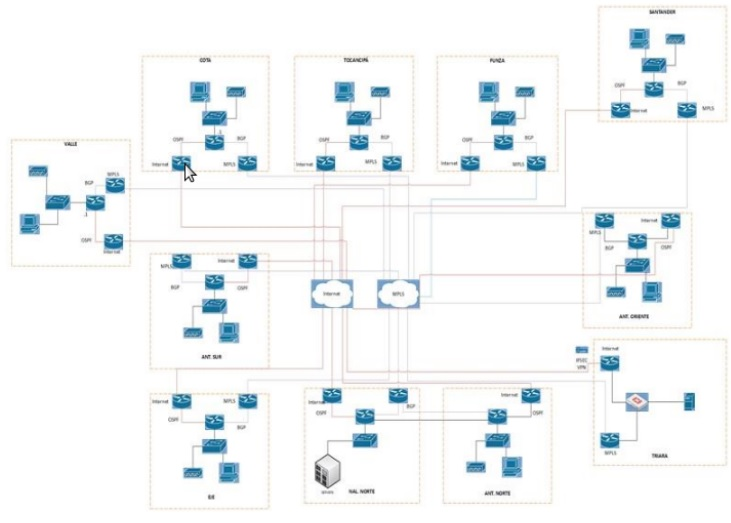
\includegraphics[width=1.0\linewidth]{figure1}}%
%  \subcaptionbox{Another sub-figure\label{fig:rightsubfig}}%
%    {
\includegraphics[width=0.5\linewidth]{knitting-vectorial}}%
 \caption{\footnotesize{Caracteríticas de un red SD-WAN}}
  \label{fig:sd-wan}
\end{figure}
\\
Se identifican como causas de los inconvenientes anteriormente mencionados la utilización de servicios en la nube y el hecho de que cada una de las sucursales debe enviarle el tráfico a las regionales para consumir cualquier recurso de red, inclusive si es una llamada a otra sucursal esto ha ocasionado los altos picos de tráfico sobre los canales de intranet.
\\
\\
Adicional a esto las sucursales cuentan con túneles EoIP \textbf{("en inglés Ethernet over IP")} configurados entre las sedes en caso de falla de su canal MPLS \textbf{("del inglés Multiprotocol Label Switching")}, pero los túneles son utilizados únicamente como \textit("backup"), por lo que el ancho de banda de los canales de internet no es utilizado aún cuando se presentan picos de saturación sobre la intranet.
\\
\\ 
Por otro lado la causa de la lentitud en la configuración de nuevas políticas o servicios de red es el hecho de que los cambios se realizan manualmente, es por este motivo que dentro de la solución se propondrá el hecho de que haya gestión centralizada desde la controladora SD-WAN \textbf{(“Software Defined Networking in Wide Area Networks”)}. En cuanto a los problemas de seguridad presentados se incluye dentro de la solución el cifrado de los túneles que interconectan tanto las sucursales como las oficinas regionales, de manera que el tráfico deje de cursar en texto claro por la red pública.
\\
\\
Por otro lado una de las causas más importantes de los problemas de disponibilidad de servicio que ha presentado el cliente ha sido que bajo el modelo actual la conmutación de sus servicios de DataCenter se realiza a través de unas VPN \textbf{(en inglés Virtual Private Network)} IPSEC \textbf{("abreviatura de Internet Protocol security")} que se suben manualmente en los equipos, lo que incrementa el tiempo de indisponibilidad de los servicios y los tiempos de gestión de fallas.
\\
\\
\textbf{Punto de Equilibrio:} el servicio es el medio a través el Diseño de la red e implementación con una SD-WAN, satisface las necesidades del cliente, materializando o dando respuesta a las necesidades reales que esta presentando. Como sabemos es necesario tratar de cubrir o sastifaces lo que el usuario necesita, en la medida que el servicio prestado mejor en calidad. A partir de que mejore el servicio de red, se define una estrategía de Marketing, es decir se vuelve adecuado para los clientes adquiriendo un precio alto, promoción y atractivo, se pone en manifiesto la importancia de la combinación y el equilibrio entre servicio y negocio.

\section{Aspectos a Solucionar} % (fold)
\label{sec:Aspectos a Solucionar}

La gestión de la infraestructura de red debe realizar de forma manual en cada una de las tiendas.
\\
	La comunicación por internet entre las diferentes regionales se realiza sin cifrar y la de las tiendas se cifra bajo un protocolo que ya no es considerado seguro.
\\
	La conexión hacia el centro de datos no cuenta con un respaldo automático sino que en este momento debe realizarse de forma manual lo cual aumenta el tiempo de gestión de una falla y por lo tanto disminuye el tiempo de disponibilidad.
\\
	En momentos de congestión de la red el tráfico cursa únicamente por el canal principal de la MPLS \textbf{("del inglés Multiprotocol Label Switching")} y el ancho de banda disponible por el canal de internet no es aprovechado.
\\
La conexión de las tiendas hacia todos los servicios que consume depende del canal de internet de la regional, si este se cae todas las tiendas que están asociadas a él quedan sin conexión.


\begin{table}[ht]
\caption{Tabla de Aspectos a Solucionar de una Red Tradicional a SD-WAN}
\label{tabla:autores}
\centering
\begin{tabular}{p{3.5cm} p{5.5cm} p{5.5cm} }
\hline
\textbf{Caractéristicas} & \textbf{Red Actual} & \textbf{Implementación SD-WAN} \\
\hline
\textbf{Gestión} &  La Gestión de infraestructura se realiza de forma Manual.  & Se tiene un gestor de Administración facilitando lo relacionado con la infraestructura.\\
\hline
\textbf{Cifrado} & El tipo de cifrado utilizado no es seguro, abriendo brechas a vulnerabilidades. & Mayor cifrado y utilización de protocolos seguros . \\
\hline
\textbf{Tráfico} & Congestión de Tráfico & Balanceo de tráfico, permite distribución del mismo. \\
\hline
\textbf{Red} & Si exite caída de una red Regional, puede afectar las demás sedes generando lentitud y caída en toda la red. & Si existe caída en una región, solo afecta a esta misma y no a las demás subredes. \\
\hline

\end{tabular}
\end{table}


\section{Solución Propuesta} % (fold)
\label{sec:Solución Propuesta}

Se propone realizar un diseño para el cambio de esquema de conectividad WAN \textbf{("Wide Area Network en inglés")} del cliente de una solución tradicional a una solución SD-WAN \textbf{(“Software Defined Networking in Wide Area Networks”)} que permita realizar los cambios de forma centralizada y más ágil, esta automatización debe realizarse en conjunto con políticas de conectividad que le garanticen al cliente el balanceo de carga del tráfico WAN \textbf{("Wide Area Network en inglés")} de manera eficiente e inteligente utilizando los enlaces dependiendo de las necesidades del tráfico de cada aplicación.
\\
\\
	La solución debe incluir además un esquema de transporte que de independencia del medio o servicio que se utilice (Internet o Intranet) y que permita tanta flexibilidad de cambiar el tipo de servicio de manera transparente cómo reducir los costos mensuales del cliente en cuanto a enlaces WAN \textbf{("Wide Area Network en inglés")}, esto debe realizarse con el protocolo de enrutamiento que más se ajuste al esquema y con las políticas de QoS \textbf{Calidad de Servicio} necesarias para garantizar que el tráfico de cada servicio funcione de forma adecuada.
\\
\\
	La solución debe diseñarse además de forma que todos los aspectos mencionados anteriormente apliquen tanto para el tráfico que el cliente utilice para aplicaciones en la nube como para el que se encuentren en DataCenter administrado por ellos o en el centro de datos del ISP \textbf{(" en inglés de Internet service provider")}.
\\
\\
	El cliente requiere por tanto una solución de SD-WAN \textbf{(“Software Defined Networking in Wide Area Networks”)} que disminuya los costos de la operación y al mismo tiempo incremente la disponibilidad de ancho de banda y eficiencia de sus conexiones WAN \textbf{("Wide Area Network en inglés")} mediante un balanceo de carga entre sus enlaces principal y de respaldo. El cliente requiere que cumpla con los siguientes criterios:

\begin{itemize}
\item[•] \textbf{Balanceo de Tráfico Inteligente:} el cliente requiere que sea utilizado el ancho de banda de los dos canales que tiene en cada sede para soportar la cantidad de tráfico que implica su migración de servicios a la nube, este balanceo debe ser inteligente de manera que se cumpla con los requisitos de retardo, \textit{"jitter"} y pérdida de paquetes que requiere cada aplicación de la compañía, si estos criterios no se cumplen bajo uno de los canales el tráfico debe ser enviado por el otro de forma automática.

\item[•] \textbf{Seguridad:} al tratarse de tráfico transaccional el cliente requiere que el transporte de datos cumpla con todos los requisitos de seguridad en la compañía en cuanto a la integridad, privacidad y disponibilidad.

\item[•] \textbf{Disponibilidad:} se requiere que el servicio tenga una alta disponibilidad y que esta se priorice para las aplicaciones críticas del cliente, el esquema de alta disponibilidad debe ser automático.

\item[•] \textbf{Aprovisionamiento Ágil:} se requiere que en caso de requerir cambios generales a nivel de red WAN \textbf{("Wide Area Network en inglés")} estos no tengan que ser configurados de forma manual en cada una de las sedes, sino que por el contrario puedan configurarse políticas de forma centralizada y enviarse las configuraciones de forma masiva para agilizar la implementación de cambios.

\item[•] \textbf{Independencia del Transporte:} se requiere una solución que no dependa de la forma de transporte, que pueda establecerse por internet o por MPLS \textbf{("del inglés Multiprotocol Label Switching")}sin inconvenientes y que si se decide cambiar de tecnología esto sea transparente para el servicio.

\item[•] \textbf{Adecuado para Nube Híbrida:} la solución propuesta debe cumplir los requerimientos tanto para las aplicaciones que se encuentran en la nube como para aquellas que aún están en el DataCenter del cliente, y debe realizar balanceo y dar prioridad a las aplicaciones.

\item[•] \textbf{Calidad de Servicio:} el diseño debe tener unas políticas de QoS \textbf{(Calidad de Servicio)} que garanticen el correcto funcionamiento de todas las aplicaciones que cursan por la red, que incluyen tráfico de voz y video.                                 

\item[•] \textbf{Conexiones Dinámicas:} el diseño propuesto debe utilizar tecnologías que eliminen la necesidad de configurar túneles estáticos cada vez que se agregue una sede o regional sino que estos se configuran dinámicamente en una tecnología en malla.
\end{itemize}

%\section{Metodología} % (fold)
%\label{sec:Metodología}


%\section{Contribuciones} % (fold)
%\label{sec:Contribuciones}

%\section{Estructura de la Tesis} % (fold)
%\label{sec:Estructura de la Tesis}